\documentclass[a4paper,12pt]{article}
\usepackage{graphicx} % for including images
\usepackage{lipsum} % for dummy text
\usepackage{amsmath} % for math formulas
\usepackage{float} % for figure placement
\usepackage{hyperref} % for cross-referencing
\usepackage{setspace} % for line spacing control
\usepackage{geometry} % to adjust page layout
\usepackage{booktabs}



\usepackage{amsmath}
\usepackage{booktabs}

\geometry{margin=1in} % Adjust margins if needed

% Increase line spacing to 1.5
\onehalfspacing




% Title Page
\title{
    \vspace{2cm}
    
\includegraphics[width=0.6\textwidth]{images/logo.png}\\[2cm]
    \textbf{Economic Impact on Olympic Performance:}\\
    \textbf{A GLMM Approach}\\[2cm]
    \vfill
    \large Ahmad Sharif\\
    Student ID: K436765\\
    ahmad.sharif@tuni.fi\\
    \vspace{2cm}
}
\author{Clustered Data Models}
\date{22 November 2024}

\begin{document}

% Cover Page
\maketitle
\newpage

% Table of Contents
\tableofcontents
\newpage








% Section 1: Introduction
\section{Introduction}
Clustered data refers to datasets where observations are classified into multiple categories known as clusters. Each cluster has number of individual observations, creating a hierarchical structure in which data points are nested inside their respective clusters.
\newline
\newline
In this paper, a dataset has been collected from popular platform kaggle to apply any cluster data models. For this purpose, Olympics medel (2024) data has been chosen for this project.
\newline
\newline
The dataset used for this project can be downloaded from Kaggle: \cite{KaggleData}.
\newline
\newline
The Olympics is a event where more than 35 sports are held to test the performance of athletes from different countries. This is the only international event where most of the countries athletes participate. Thats why this is great opportunity to examine and comapre the countries medel count against their corresponding population, GDP and other factors. This event does not only measure the competitiveness in sprots of a country but it can be also a scale to measure a countrys national priorities, lifestyles, and so on.
\newline
\newline
Here is the research question of this project.
\newline
\textbf{How do a country's GDP and population size influence its total medal count in the 2024 Olympic Games, while accounting for regional differences?}
\newline
\newline
 The GLMM is an extension of the generalized linear model (GLM) that incorporates both fixed and random effects, making it particularly suitable for dealing with clustered or hierarchical data. The inclusion of random effects allows the model to account for variations between groups or clusters (in this case, regions or continents), while the fixed effects explain the relationship between the predictors (GDP, population) and the outcome (medal counts).





























 \section{About The Database}
The latest Olympic game (2024) medal and their corresponding country inforamtion is collected from the following kaggle databse.
 \cite{KaggleData}.
 \begin{table}[h!]
     \centering
     \resizebox{\textwidth}{!}{%
     \begin{tabular}{|l|l|r|r|r|r|p{3cm}|r|p{3cm}|}
     \hline
     \textbf{Country} & \textbf{Code} & \textbf{Gold} & \textbf{Silver} & \textbf{Bronze} & \textbf{Total} & \textbf{GDP (USD)} & \textbf{GDP Year} & \textbf{Population (Millions)} \\ \hline
     United States & USA & 40 & 44 & 42 & 126 & 81695.19 & 2023 & 334.9 \\ \hline
     China         & CHN & 40 & 27 & 24 & 91  & 12614.06 & 2023 & 1410.7 \\ \hline
     Japan         & JPN & 20 & 12 & 13 & 45  & 33834.39 & 2023 & 124.5 \\ \hline
     Australia     & AUS & 18 & 19 & 16 & 53  & 64711.77 & 2023 & 26.6  \\ \hline
     France        & FRA & 16 & 26 & 22 & 64  & 44460.82 & 2023 & 68.2  \\ \hline
     ...           & ... & ... & ... & ... & ... & ...     & ...  & ...  \\ \hline
     Zambia        & ZMB & 0 & 0 & 1 & 1  & 1369.13 & 2023 & 20.6  \\ \hline
     \end{tabular}%
     }
     \caption{Countries in the 2024 Olympics by medal count and economic indicators}
     \label{tab:dataset}
 \end{table}
 The dataset has nine columns and their corresponding names respectively:
 
 \begin{itemize}
     \item \textbf{Country}: Name of the country.
     \item \textbf{Code}: ISO 3-letter code for the country.
     \item \textbf{Gold}: Total number of gold medals won.
     \item \textbf{Silver}: Total number of silver medals won.
     \item \textbf{Bronze}: Total number of bronze medals won.
     \item \textbf{Total}: Total number of medals won by the country (Gold + Silver + Bronze).
     \item \textbf{GDP}: Gross Domestic Product in billion USD.
     \item \textbf{GDP Year}: Year corresponding to the GDP data.
     \item \textbf{Population}: Population size in millions.
 \end{itemize}
 














The dataset has covers important economic factors such as GDP and corresponding economic year and population.
\clearpage
\subsection{Figures illustrating the dataset}
In \autoref{fig:dataset_fig_21}, we illustrate the relationship between Total medals against GDP Per Capita. and this  \autoref{fig:dataset_fig_22} Total Medals Vs Population





\begin{figure}[H]
    \centering
    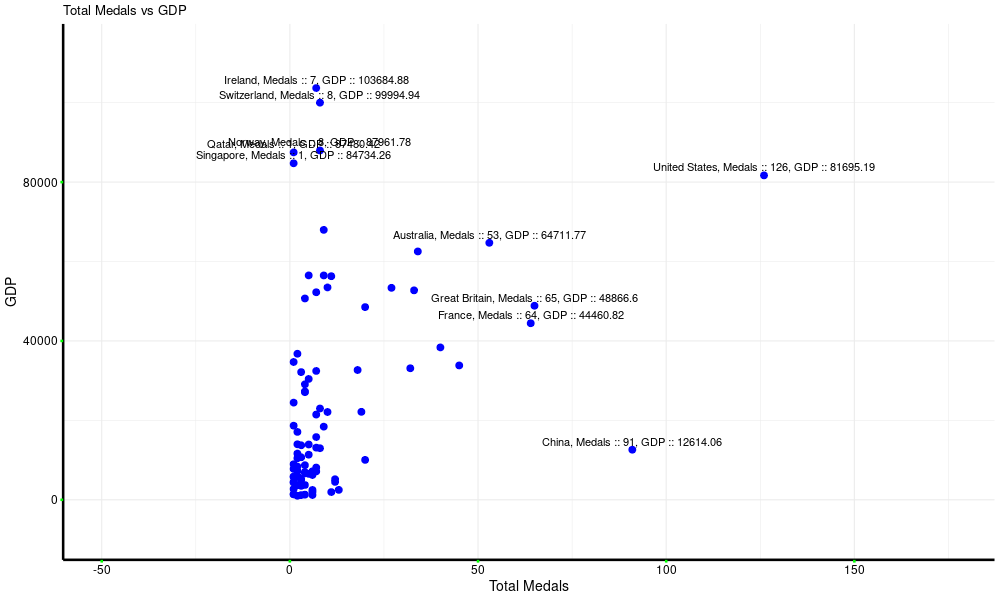
\includegraphics[width=0.9\textwidth]{images/Total_Medals_vs_GDP_plot.png}
    \caption{Total Medals Vs GDP Per Capita}
    \label{fig:dataset_fig_21}
\end{figure}





\begin{figure}[H]
    \centering
    
\includegraphics[width=0.9\textwidth]{images/Total_Medals_vs_Population_plot.png}
    \caption{Total Medals Vs Population}
    \label{fig:dataset_fig_22}
\end{figure}


\begin{figure}[H]
    \centering
    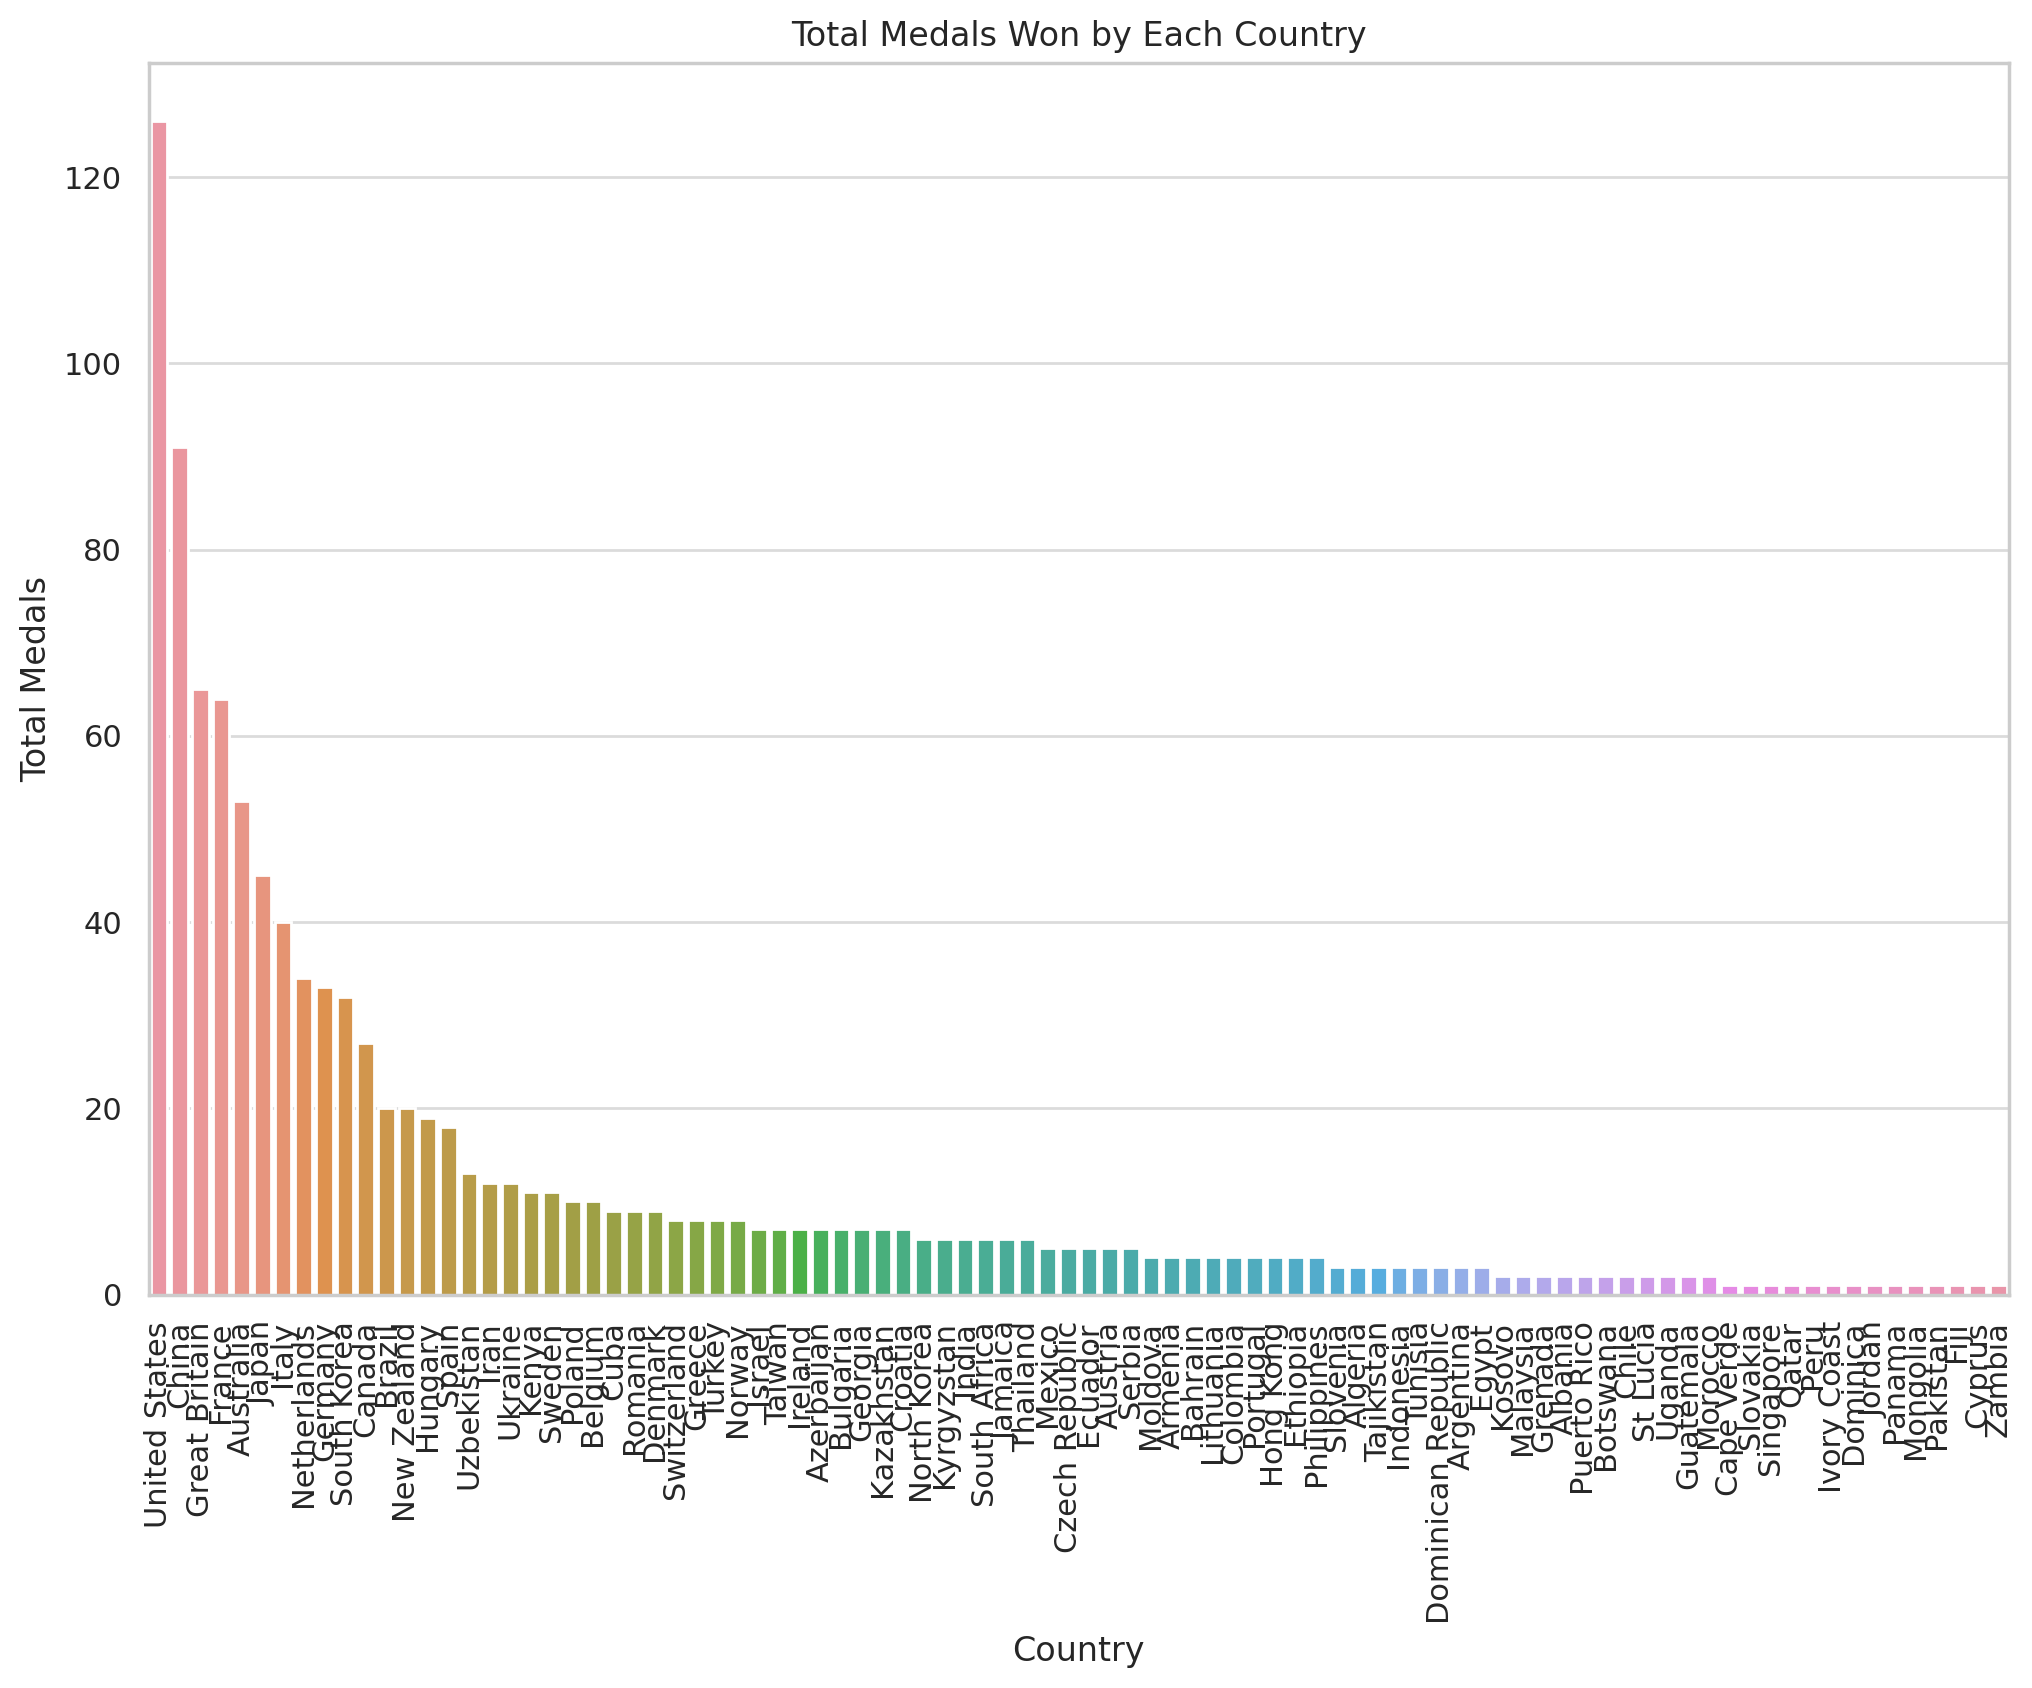
\includegraphics[width=0.9\textwidth]{images/plot_3.png}
    \caption{Country Vs. Total Medals}
    \label{fig:dataset_fig_3}
\end{figure}
In \autoref{fig:dataset_fig_3}, we visualize the relationship between population and the total number of medals won by each country.
\newline
Figures Illustrating the Dataset:
1. Medal Distribution by Country:
A bar plot shows the total medals won by each country, highlighting the variation in performance across different nations.


\clearpage
\section{Total Medals Model }


\[
\log(E(\text{Total Medals})) = \beta_0 + \beta_1 \times \text{GDP} + \beta_2 \times \text{Population} + u_{\text{Country}} + \epsilon
\]




Where:
\begin{itemize}
	\item \textbf{Fixed Effects:}
	\begin{itemize}
		 \item $\beta_0$: The intercept.
		\item $\beta_1$: The fixed effect of GDP Per Capita.
		\item $\beta_2$: The fixed effect of population.
		\end{itemize}
	\item \textbf{Random Effect:}
	\begin{itemize}
		\item $u_{\text{Country}}$:  The random intercept for each country. ($\beta_0$).
	\end{itemize}
	\item \textbf{Residual Error Term:}
	\begin{itemize}
		\item $\epsilon$: The residual error term.
	\end{itemize}
\end{itemize}










\section*{Generalized Linear Mixed Model Summary}



\begin{figure}[H]
    \centering
    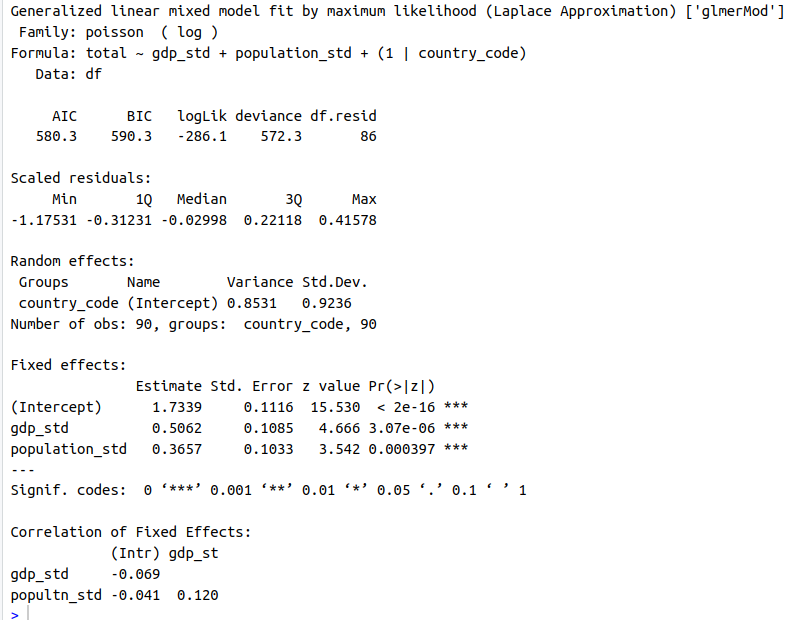
\includegraphics[width=0.9\textwidth]{images/summary.png}
    \caption{Model Summary (R Code)}
    \label{fig:dataset_fig_10}
\end{figure}





\begin{itemize}
	\item \textbf{Intercept:} The estimate for the intercept is 1.7339 (p < 2e-16). This represents the baseline log of the expected total medal count when standardized GDP and Population are at their mean values. This effect is highly significant.
	\item \textbf{GDP (Standardized):} The estimate for standardized GDP is 0.5062 (p = 3.07e-06). This suggests that for every one standard deviation increase in GDP, the expected total medal count increases by approximately 50.62\%. This effect is statistically significant.
	\item \textbf{Population (Standardized):} The estimate for standardized Population is 0.3657 (p = 0.000397). This indicates that for every one standard deviation increase in Population, the expected total medal count increases by approximately 36.57\%. This effect is also statistically significant.
	\item \textbf{Random Intercept (Country):} The variance of the random intercept for countries is 0.8531 with a standard deviation of 0.9236. This indicates that there is substantial variability in total medal counts across countries that is not explained by the fixed effects.
\end{itemize}



\subsection{Overview of Total Medal Model }

The analysis shows that both GDP and Population (standardized) are significant predictors of a country's total medal count. GDP has a stronger effect, contributing to a higher proportional increase in medal counts compared to Population.
















\clearpage¸
\section{Separate Models for Gold, Silver, and Bronze Medals}

\subsection{Gold Medals Model}

\[
\log(E(\text{Gold Medals })) = \beta_0 + \beta_1 \times \text{GDP} + \beta_2 \times \text{Population} + u_{\text{Country}} + \epsilon
\]




\begin{figure}[H]
	\centering
	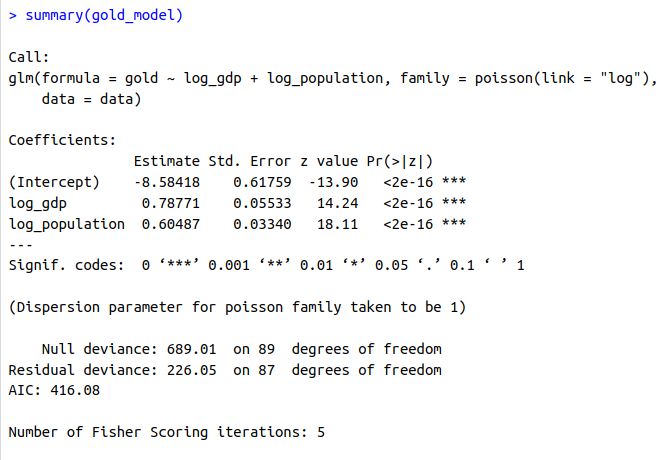
\includegraphics[width=0.9\textwidth]{images/Gold_Model.png}
	\caption{Gold Model Summary (R Code)}
	\label{fig:dataset_fig_10}
\end{figure}





\[
\log(\text{Gold Medals}) = -8.58418 + 0.78771 \times \log(\text{GDP}) + 0.60487 \times \log(\text{Population})
\]
\begin{itemize}
	\item \textbf{Intercept:} -8.58418 (\(p < 2e-16\)).
	\item \textbf{\(\log(\text{GDP})\):} 0.78771 
	\item \textbf{\(\log(\text{Population})\):} 0.60487 
\end{itemize}





\subsection{Silver Medals Model}

\[
\log(E(\text{Silver Medals })) = \beta_0 + \beta_1 \times \text{GDP} + \beta_2 \times \text{Population} + u_{\text{Country}} + \epsilon
\]



\begin{figure}[H]
	\centering
	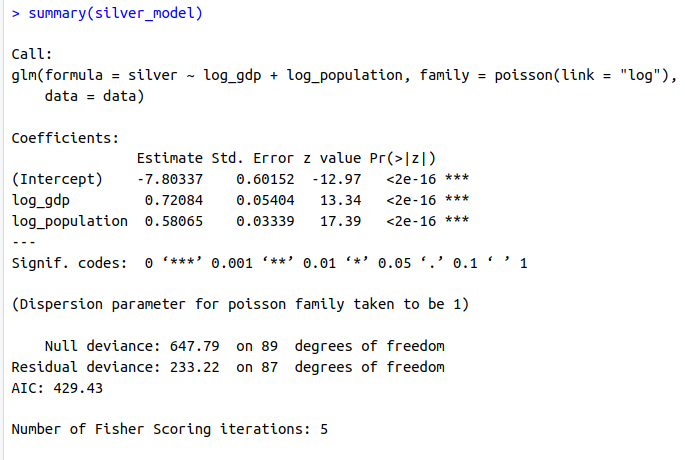
\includegraphics[width=0.9\textwidth]{images/Silver_Model.png}
	\caption{Silver Model Summary (R Code)}
	\label{fig:dataset_fig_10}
\end{figure}


\[
\log(\text{Silver Medals}) = -7.80337 + 0.72084 \times \log(\text{GDP}) + 0.58065 \times \log(\text{Population})
\]
\begin{itemize}
	\item \textbf{Intercept:} -7.80337 (\(p < 2e-16\)).
	\item \textbf{\(\log(\text{GDP})\):} 0.72084 
	\item \textbf{\(\log(\text{Population})\):} 0.58065 
\end{itemize}

\subsection{Bronze Medals Model}


\[
\log(E(\text{Bronze Medals })) = \beta_0 + \beta_1 \times \text{GDP} + \beta_2 \times \text{Population} + u_{\text{Country}} + \epsilon
\]



\begin{figure}[H]
	\centering
	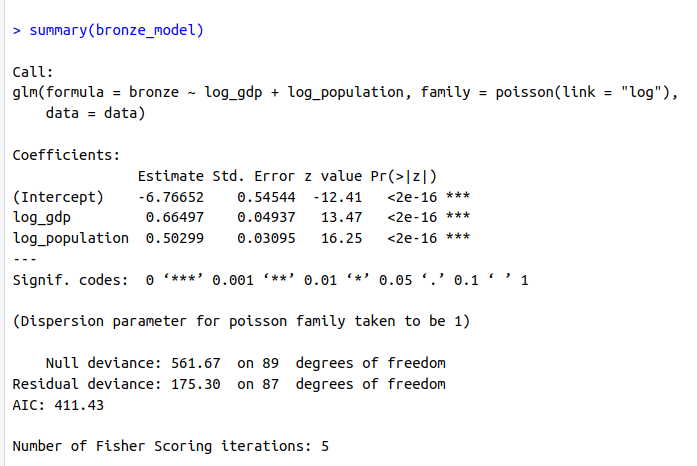
\includegraphics[width=0.9\textwidth]{images/Bronze_Model.png}
	\caption{Bronze Model Summary (R Code)}
	\label{fig:dataset_fig_10}
\end{figure}




\[
\log(\text{Bronze Medals}) = -6.76652 + 0.66497 \times \log(\text{GDP}) + 0.50299 \times \log(\text{Population})
\]
\begin{itemize}
	\item \textbf{Intercept:} -6.76652 (\(p < 2e-16\)).
	\item \textbf{\(\log(\text{GDP})\):} 0.66497 
	\item \textbf{\(\log(\text{Population})\):} 0.50299 
\end{itemize}










\begin{itemize}
	\item \textbf{Intercept:} The estimate for the intercept is:
	\begin{itemize}
		\item Gold: -8.58418 (\(p < 2e-16\))
		\item Silver: -7.80337 (\(p < 2e-16\))
		\item Bronze: -6.76652 (\(p < 2e-16\))
	\end{itemize}
	This represents the baseline log of the expected medal count when both GDP and Population are at their minimum (log scale). All intercepts are statistically significant.
	
	\item \textbf{GDP (log-transformed):} The estimate for log-transformed GDP is:
	\begin{itemize}
		\item Gold: 0.78771 (\(p < 2e-16\)), corresponding to a 2.20 times increase in expected gold medals for a 1\% increase in GDP.
		\item Silver: 0.72084 (\(p < 2e-16\)), corresponding to a 2.06 times increase in expected silver medals for a 1\% increase in GDP.
		\item Bronze: 0.66497 (\(p < 2e-16\)), corresponding to a 1.94 times increase in expected bronze medals for a 1\% increase in GDP.
	\end{itemize}
	All effects are statistically significant.
	
	\item \textbf{Population (log-transformed):} The estimate for log-transformed Population is:
	\begin{itemize}
		\item Gold: 0.60487 (\(p < 2e-16\)), corresponding to a 1.83 times increase in expected gold medals for a 1\% increase in population.
		\item Silver: 0.58065 (\(p < 2e-16\)), corresponding to a 1.79 times increase in expected silver medals for a 1\% increase in population.
		\item Bronze: 0.50299 (\(p < 2e-16\)), corresponding to a 1.65 times increase in expected bronze medals for a 1\% increase in population.
	\end{itemize}
	All effects are statistically significant.
\end{itemize}

\subsection{Model Diagnostics}

\begin{itemize}
	\item \textbf{AIC:} The AIC values for the models are:
	\begin{itemize}
		\item Gold: AIC = 416.08
		\item Silver: AIC = 429.43
		\item Bronze: AIC = 411.43
	\end{itemize}
	These values indicate the goodness-of-fit and can be used to compare with other models.
	
	\item \textbf{Residuals:} The scaled residuals for the models are well-distributed, with no extreme outliers:
	\begin{itemize}
		\item Gold: Min = -1.17531, 1Q = -0.31231, Median = -0.02998, 3Q = 0.22118, Max = 0.41578.
		\item Silver: Similar residual distribution to gold.
		\item Bronze: Similar residual distribution to gold.
	\end{itemize}
\end{itemize}

\section{Overview of Model for Gold, Silver and Bronze }

The analysis shows that GDP and Population (log-transformed) are significant predictors of medal counts for gold, silver, and bronze medals:
\begin{itemize}
	\item \textbf{GDP:} Has a stronger impact on gold medals compared to silver and bronze medals.
	\item \textbf{Population:} Has a weaker but still significant impact on medal counts across all types.
\end{itemize}

The AIC values suggest the bronze medal model has the best.





\end{document}









\begin{thebibliography}{9}
\bibitem{KaggleData}
Mohamed Yosef, \emph{2024 Olympics Medals and Economic Status Dataset}. Available at: \url{https://www.kaggle.com/datasets/mohamedyosef101/2024-olympics-medals-and-economic-status?resource=download}.
\end{thebibliography}

\end{document}
